\chapter{Project Setup}\label{ch:project_setup}
This chapter will describe the project's data sources and the Python library \emph{spacy}, which was extensively used for the \gls{ner} and \gls{coref_resolution_definition} components in the \emph{Information Extraction Pipeline}.

\section{Data}\label{sec:data}
The data consists of \emph{News Articles} and \emph{Company Data}.
The dataset requirements are derived from the project's domain focus as outlined in section \ref{sec:domain-focus}.
This requires that
\begin{itemize}
	\item news articles must be in German language.
	\item news articles should mention companies, at least potentially.
	\item companies must be publicly listed on a stock exchange.
	\item companies must be based in Europe.
    \item such company and news articles data must be publicly available.
\end{itemize}

\subsection{News Articles}
Many news article datasets are available on platforms such as Kaggle \cite{kaggle}, but it seems that only a few of them are in German \cite{kaggle}.
Most of the German news datasets that I analyzed are either not rooted in the financial domain, outdated for copyright reasons or
deal with macroeconomic policies or broader economic trends rather than company news.\\

As I could not find proper data that fits the outlined objectives, I decided to scrape the information from financial news providers.

\paragraph{Sources}\label{par:sources}
The data was scraped from the websites of \emph{EQS-News} \cite{WebsiteEQSNews} and \emph{dpa-AFX} \cite{WebsiteDPAAFX}, both business news hubs that aggregate multiple news sources.
The text in the html-files were converted to text files, cleaned and read into pandas \cite{pandas} DataFrames.
The type of the news articles includes \emph{ad-hoc news}, \emph{press releases}, \emph{corporate news} and \emph{regulatory filings}.
These could be published by \emph{companies} themselves or \emph{media outlets} such as newspapers, news agencies or other broadcasters.

\paragraph{Data Description}\label{par:data-description}
Of the news articles, the article text, the article title and some other metadata such as publication dates, authors, etc. were scraped.
The news articles contained many irregularities, errors, misspellings and phrases that were not part of the actual news.\\
Multiple regular expression (\gls{Regex}) patterns and techniques were applied to clean the text.
Most of the errors and undesired phrases of the text could be removed, but not all.
So the subsequent models must handle them.\\
The news article dates range from \emph{May 1, 2023} through \emph{May 31, 2024} and its frequency is daily.
The daily data was aggregated on a monthly basis and the pandas DataFrames were stored as Apache parquet \cite{parquet} files.

\subsection{Company Data}
OpenBB \cite{openbb} is an open source framework that aspires to replicate the functionalities of the Bloomberg Terminal, a costly financial service product by the media company Bloomberg \cite{bloomberg}.
OpenBB offers a wide range of functionalities, connects data providers and is the data source for the company data used in the project.
Data for companies, that are publicly listed on bourses in
\begin{itemize}
    \item France
    \item Germany
    \item Great Britain
    \item Spain
    \item Italy
    \item The Netherlands
\end{itemize}
and that are members of the main stock indexes there, were downloaded and stored in an Apache parqet file.
This file contains unique company names and their stock ticker symbols for slightly above 2500 companies.

\section{Spacy}\label{subsec:spacy}
Spacy \cite{spacy} is a modular, open-source Python library that is commonly used for a wide range of \gls{nlp}-related tasks.
For popular languages like English and German, spacy offers pre-trained pipelines (see Fig.\ref{fig:spacy-pipeline}) in different sizes and versions.
\begin{figure}[H]
	\centering
	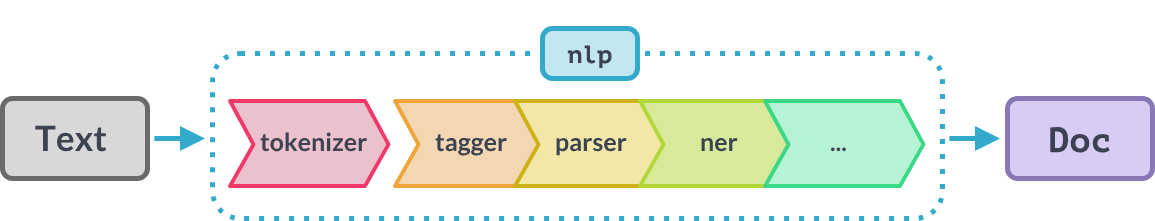
\includegraphics[width=1.0\textwidth]{Assets/spacypipe}
	\caption{\textit{Spacy Pipeline}}
	\label{fig:spacy-pipeline}
\end{figure}

The model sizes range from \emph{Small} to \emph{Medium} and \emph{Large}, with bigger models usually performing better than smaller ones.

The spacy-trained Transformer model for English is based on \gls{ROBERTA} \cite{roberta}, the one for German on \gls{BERT}-German \cite{BERT}.
The TOK2VEC \cite{spacy} embeddings for the non-Transformer models (suffixes: sm, md, lg) are memory-efficient Multi-Hash embeddings \cite{spacyembeddings} with a \gls{cnn} encoding layer \cite{spacy}.

\paragraph{Pipeline Components}
After downloading the models, by default, the modular pipeline consists of a:

\begin{itemize}
  \item \textbf{Tokenizer}: Segments text into tokens
  \item \textbf{POS-Tagger}: Assigns \gls{pos} tags such as \textit{NOUN} or \textit{VERB}
  \item \textbf{Dependency-Parser}: Assigns syntactic dependency labels between \gls{pos}-tags and sets sentence boundaries
  \item \textbf{Lemmatizer}: Assigns base forms or lemmas (see: \gls{lemmatization})
  \item \textbf{Entity-Recognizer}: Detects and labels named entities such as \gls{org} or \gls{per}
  \item \textbf{Custom Components}: Proprietary components implemented by the user
  \item \textbf{Pipeline Plugins}: External applications that are developed by others as a spacy pipeline component
\end{itemize}

The \emph{Dependency-Parser} and \emph{Entity-Recognizer} modules in the pipeline were separately trained with task-specific datasets and plugged back into the pipeline \cite{spacy} (see Fig.\ref{fig:spacy-pipeline}).

\paragraph{Custom Component}
With a spacy \emph{Custom Component}, users can implement their own custom algorithms and functions.
Compared to a pure Python implementation, these \emph{Custom Components} are usually faster as they are optimized with \gls{CPython} in the background.
This functionality was extensively used in the project as the \gls{ner} and \gls{coref_resolution_definition} pipeline components (see Fig.\ref{fig:infoextract}) were implemented with such \emph{Custom Components}.

\paragraph{Pipeline Plugins}\label{par:spacy-plugin}
Spacy \emph{Pipeline Plugins} are applications and standalone packages that are developed by other software developers to be used as a spacy pipeline component.
Such registered plugins enhance the spacy ecosystem and can easily be added by referencing it in the \textit{add\_pipe()}-function.
One such plugin studied in the project is the package \emph{Crosslingual-Coreference} ("xx\_coref") \cite{xxCoref} that was loaded with the
\begin{center}
\emph{nlp.add\_pipe("xx\_coref")}
\end{center}
function.

\paragraph{Custom Extensions}
Users can also attach custom extensions to spacy's \glspl{token} and \glspl{span} in a \emph{Doc}-Object (see Fig.\ref{fig:spacy-pipeline}) which allows them to tag or label certain words or expressions in the text to further process them later.
In the project, such custom extensions were also used extensively.
For instance: For a company identified in the \gls{span} or \gls{token} of a document (\emph{Doc}-object), the company name and company symbol (stock tocker symbol) were attached to the custom extensions \emph{comp\_name} and \emph{comp\_symbol} as in the following example:

\begin{center}
    \emph{doc.\_.comp\_name = "Adidas AG"}
\end{center}
\begin{center}
    \emph{doc.\_.comp\_symbol = "ADS.DE"}
\end{center}

Later on, all companies in a \textit{Doc}-object can be collected and further processed.

\paragraph{Modularity and Custom Pipeline}
The \emph{Tokenizer}-component is always required in the pipeline, but all other components (see Fig.\ref{fig:spacy-pipeline}) can easily be removed from it if they are not needed for a specific \gls{nlp}-task.
For instance, if only a \gls{pos}-tagger is needed to identify \emph{Nouns}, it can be enabled with the \emph{select\_pipes()}-method which also disables all other components except for the \emph{Tokenizer}:

\begin{center}
\emph{nlp.select\_pipes(enable="tagger")}
\end{center}

\subsection{Usage}\label{subsec:usage}
The spacy \emph{Custom Pipeline} was build with Python modules that can be found in the following directory:
\begin{center}
    \emph{src/B\_spacy\_pipeline}
\end{center}
In the \emph{spacy\_pipe\_build} module and \emph{SpacyPipeBuild} class, the method \emph{build\_pipe()} (Python-Code \ref{code:build-pipe}) controls the pipeline's components:

\begin{listing}[H]
    \captionof{listing}{Function: build\_pipe()}
    \inputminted[
    firstline=60,
    lastline=81,
    firstnumber=60,
    ]{python}{/media/rainergo/PROJECTS/UASFRA-MS-Thesis/src/B_spacy_pipeline/spacy_pipe_build.py}
    \label{code:build-pipe}
\end{listing}

A pipeline component can be replaced by substituting it with the desired module function depending on the specific task.
All module functions are defined in the \emph{SpacyPipeBuild} class.

\paragraph{Other Python Libraries}
Beside spacy, other important Python libraries were used, but these will be described within their particular scope in the subsequent chapters.



